Испытания представляют собой процесс установления соответствия программы и
программной документации заданным требованиям.

\subsection{Проверка требований к документации}
Проверяется наличие всех документов перечисленных в пyнкте 4.1 данного документа и их соответствие ГОСТ.

\subsection{Проверка требований к интерфейсу}
Интерфейс соответствует схеме, указанной в техническом задании. Совместим а ОС
Андроид. Использованы стандартные элементы графического семейства системы
Андроид. Используемая цветовая палитра соответствует рекомендациям сайта,
указанного в настоящем Техническом Задании.

\begin{figure}[h!]
    \centering
    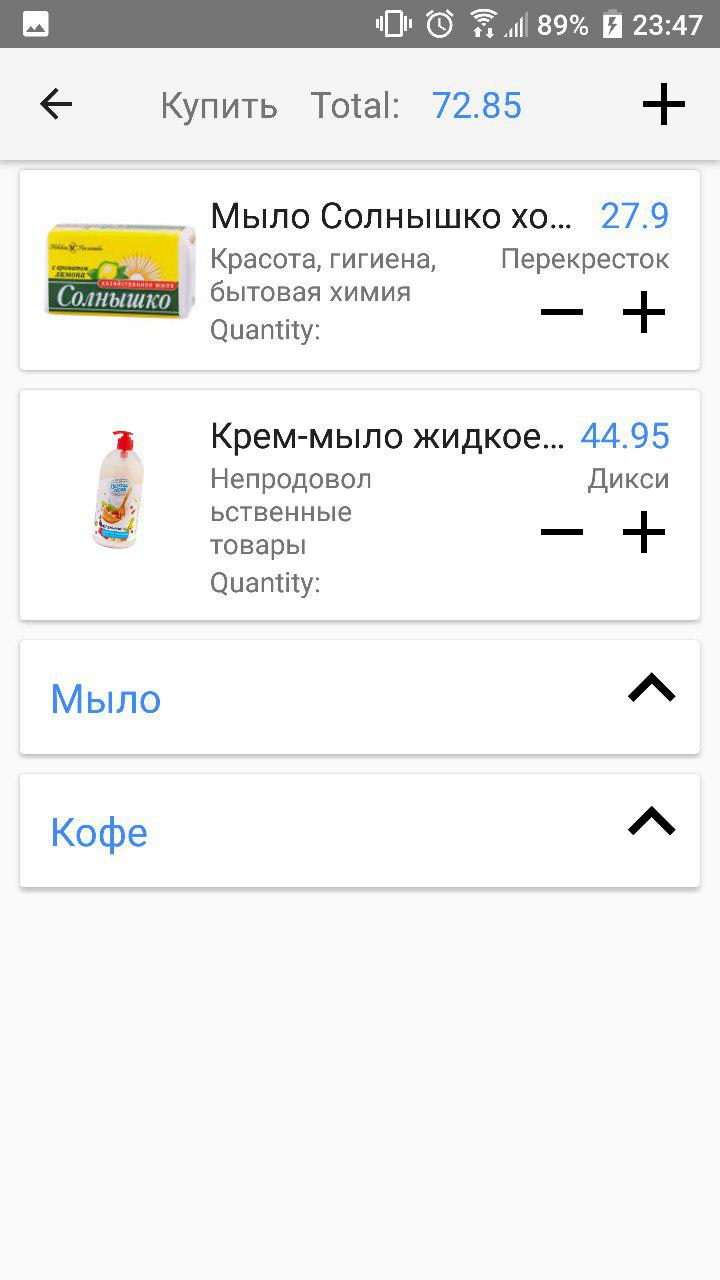
\includegraphics[height=0.48\textheight]{./screenshots/3/shoplist.jpg}
    \caption{проверка требований к интерфейсу}
\end{figure}

\newpage
\subsection{Проверка требований к функциональным характеристикам}

\subsubsection{Андроид приложение}
Реализованный функционал продемонстрирован на скриншотах ниже.

Реализованa возможность просмотра списка доступных магазинов с акционными
товарами, реализованo представление текущих акций для конкретного магазина в
виде общего списка и по категориям. Реализованa постепенная загрузкa товаров
магазинов (по страницам) для экономии трафика и меньшей нагрузкой на мобильное
устройство.

Загрузка акций не превышает лимит, установленный требованиями и проверена в пункте 6.4 настоящей Программы и Методики Испытаний.

\begin{figure}[h!]
    \centering
    \minipage{0.3\textwidth}
    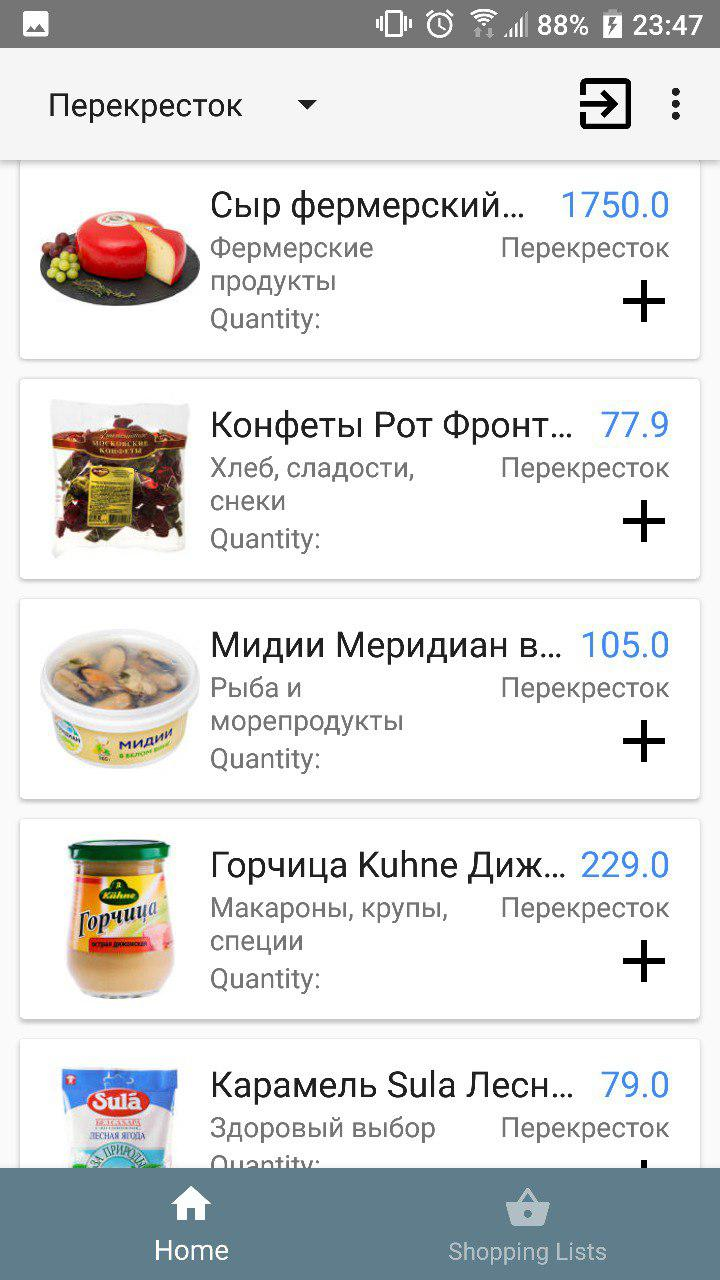
\includegraphics[height=0.38\textheight]{./screenshots/3/home.jpg}
    \caption{\small{просмотр всех акций}}
    \endminipage\hfill
    \minipage{0.3\textwidth}
    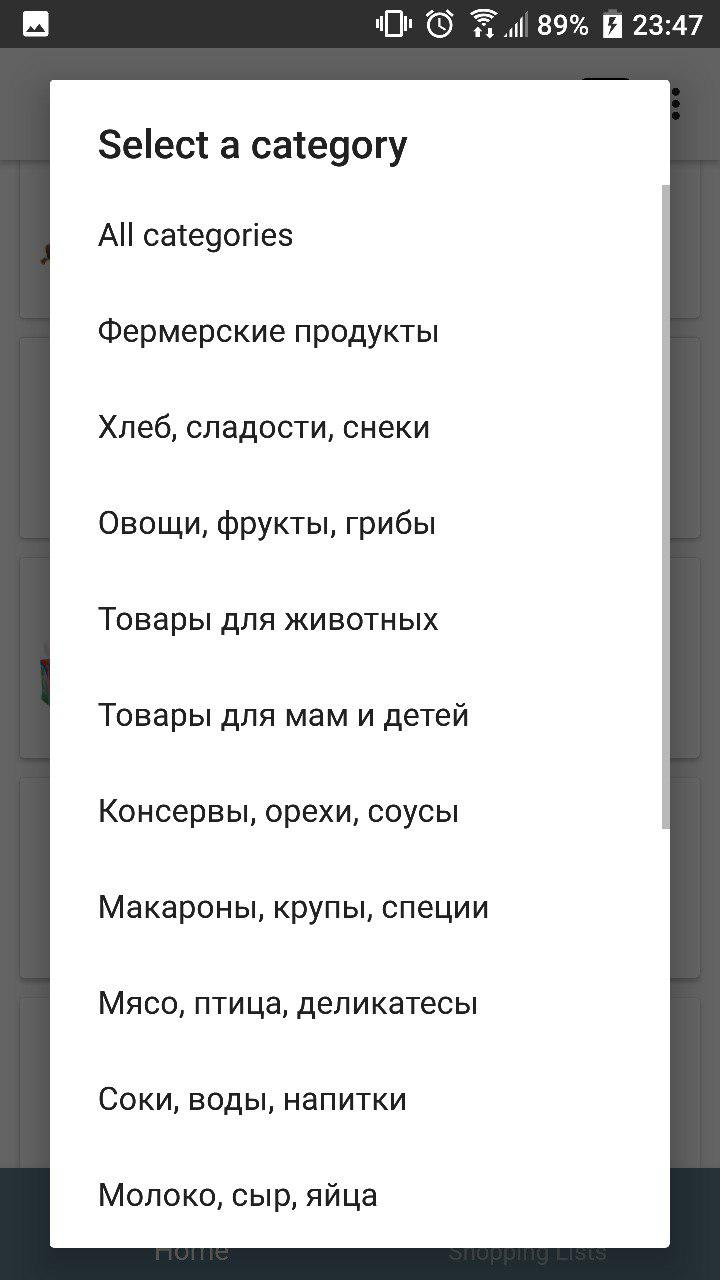
\includegraphics[height=0.38\textheight]{./screenshots/3/categories.jpg}
    \caption{\small{выбор категории}}
    \endminipage\hfill
    \minipage{0.3\textwidth}
    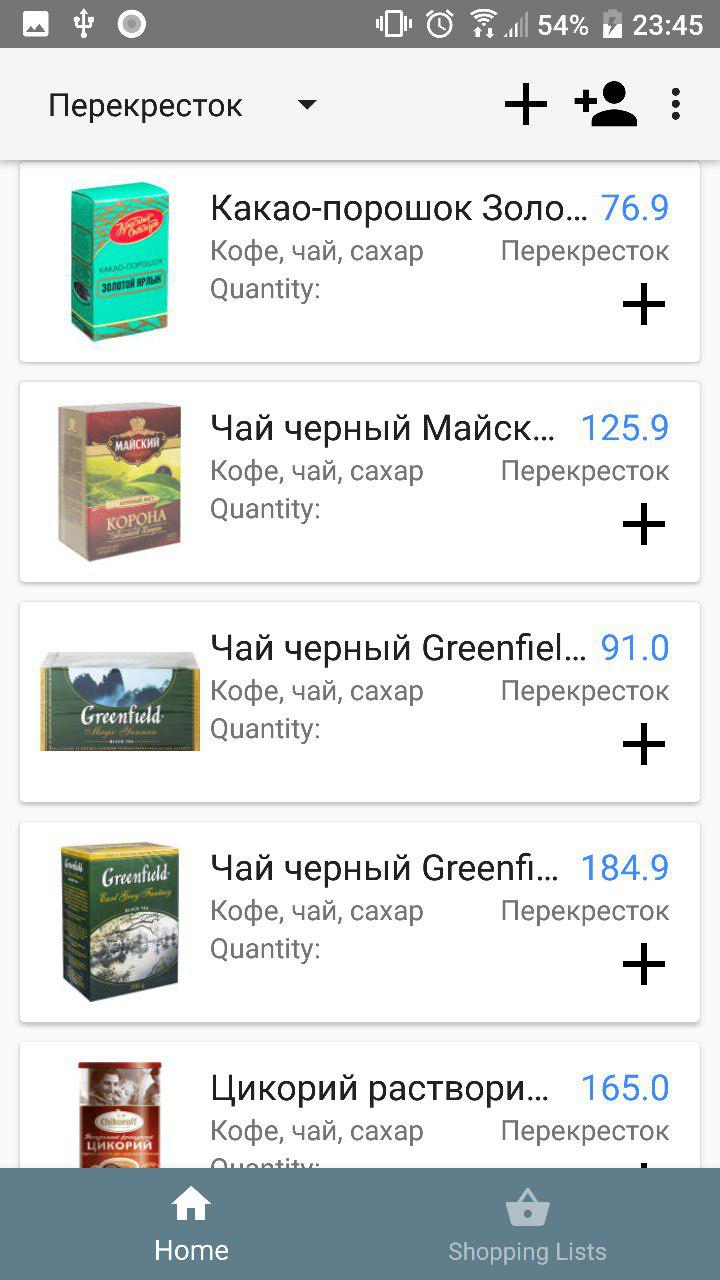
\includegraphics[height=0.38\textheight]{./screenshots/3/categ_filter.jpg}
    \caption{\small{просмотр по категориям. На скриншоте --- категория ``Кофе, чай, сахар''}}
    \endminipage{}
\end{figure}

Реализованa возможность создания списков покупок c разными названиями,
реализованa возможность удаления списка покупок.

\begin{figure}[h!]
    \centering
    \minipage{0.3\textwidth}
    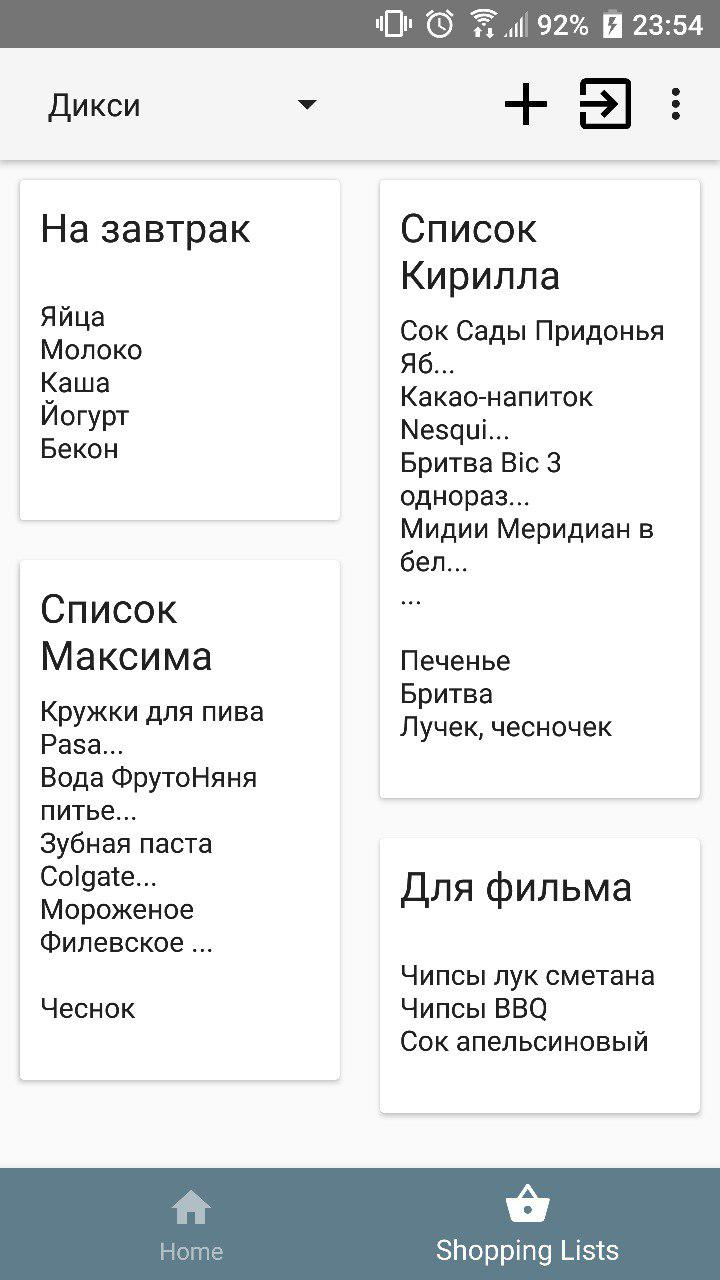
\includegraphics[height=0.38\textheight]{./screenshots/3/all_shoplists.jpg}
    \caption{\small{просмотр всех списков покупок}}
    \endminipage\hfill
    \minipage{0.3\textwidth}
    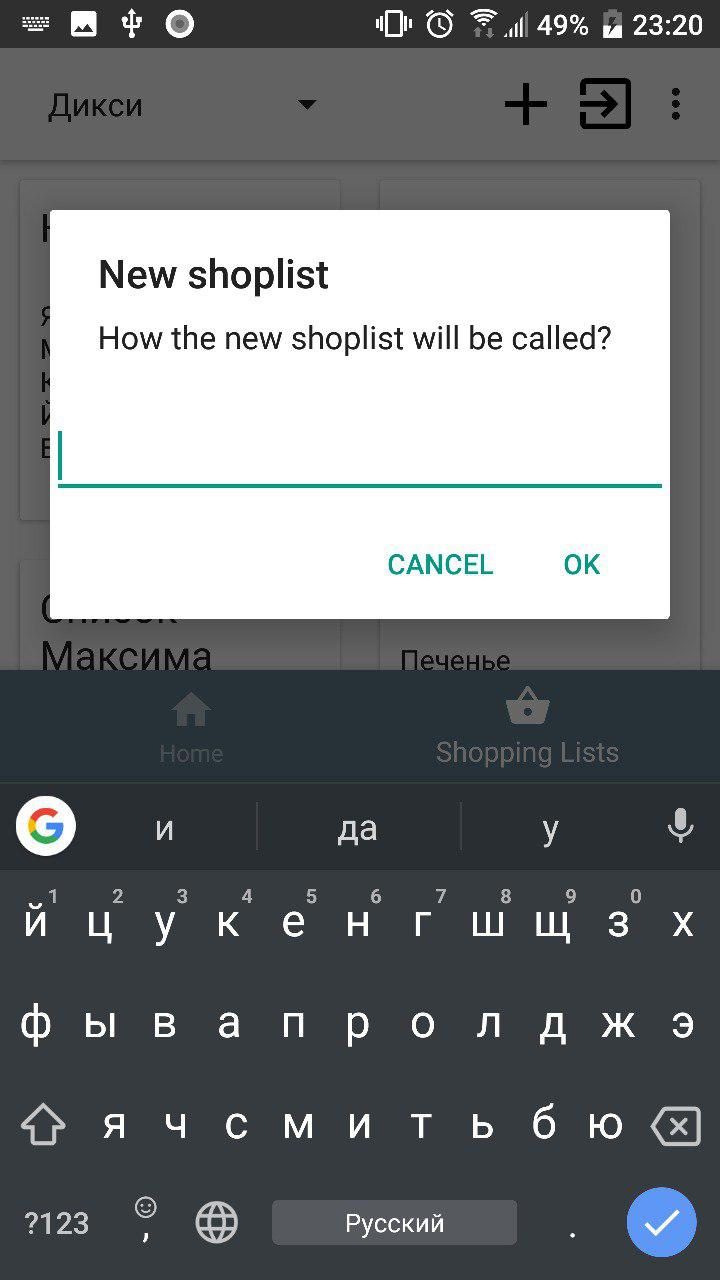
\includegraphics[height=0.38\textheight]{./screenshots/3/new_shoplist.jpg}
    \caption{\small{создание нового списка покупок}}
    \endminipage\hfill
    \minipage{0.3\textwidth}
    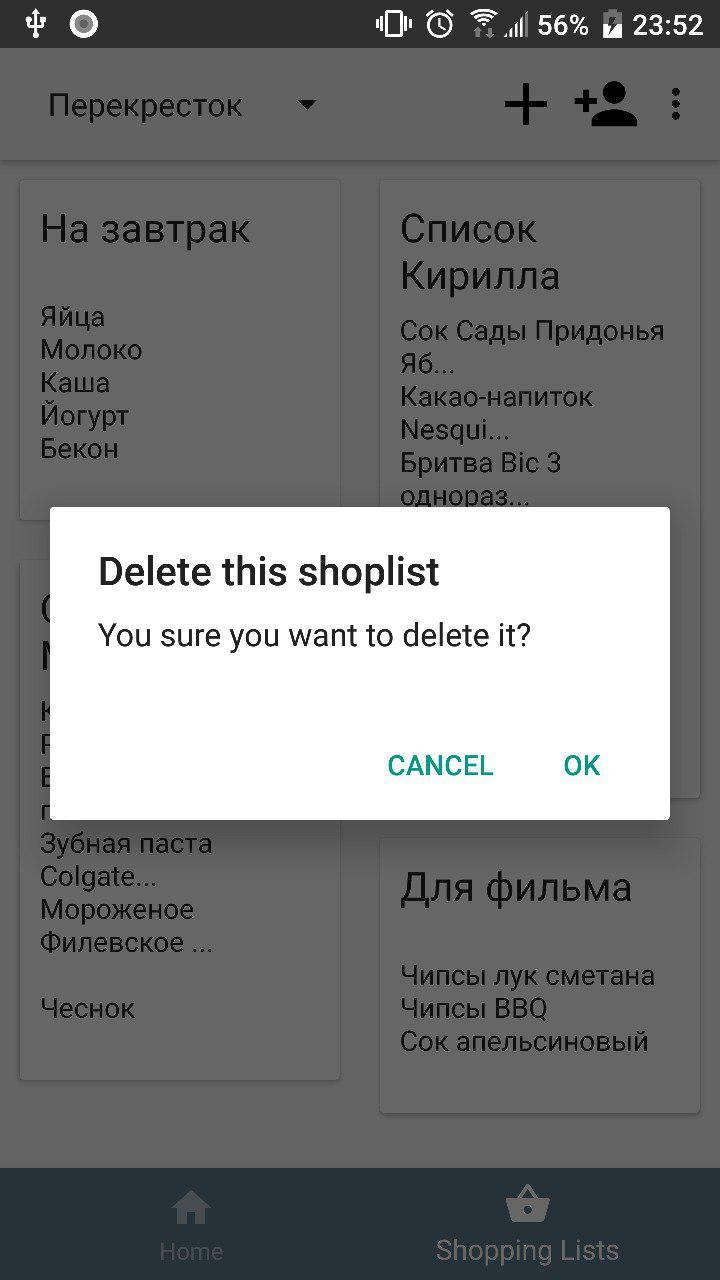
\includegraphics[height=0.38\textheight]{./screenshots/3/delete_shoplist.jpg}
    \caption{\small{удаление списка покупок}}
    \endminipage{}
\end{figure}

Реализованa возможность добавления товара в список покупок, реализованa возможность удаления товара из
списка покупок, реализованa возможность добавления в список покупок
пользовательских товаров, которых нет в магазине, pеализованa возможность
просмотра подобранных программой товаров согласно запросу пользователя,
реализовано добавление подобранных товаров в список покупок, реализовано
предварительное отображение элементов каждого списка покупок до их открытия.

\begin{figure}[h!]
    \centering
    \minipage{0.3\textwidth}
    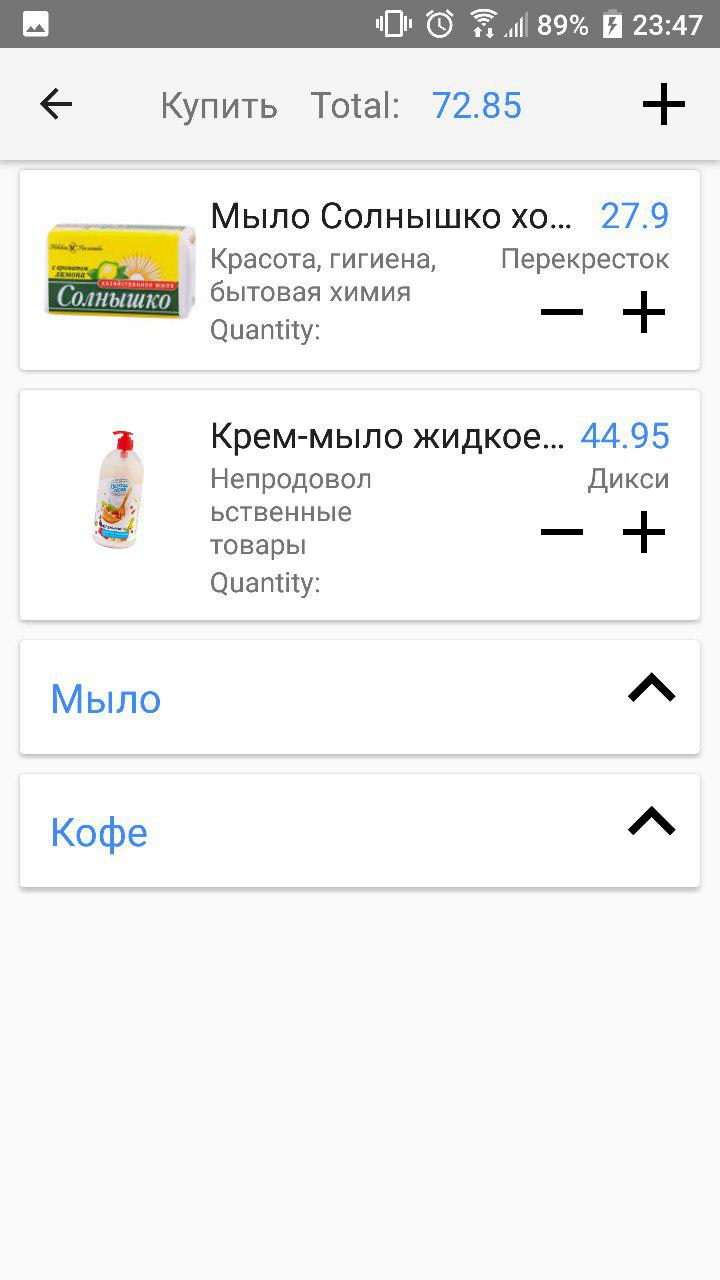
\includegraphics[height=0.38\textheight]{./screenshots/3/shoplist.jpg}
    \caption{\small{просмотр конкретного списка покупок}}
    \endminipage\hfill
    \minipage{0.3\textwidth}
    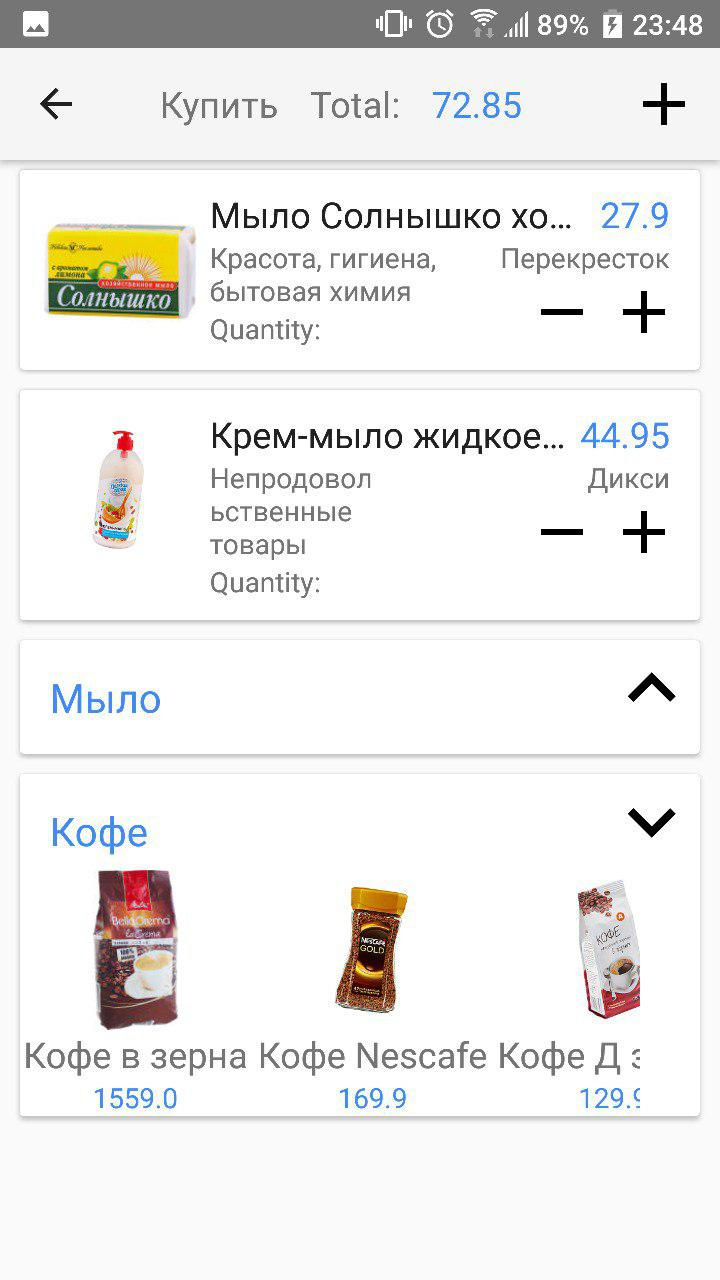
\includegraphics[height=0.38\textheight]{./screenshots/3/shoplist_custom_fold.jpg}
    \caption{\small{просмотр подобранных программой товаров в соответствии с запросом пользователя}}
    \endminipage\hfill
    \minipage{0.3\textwidth}
    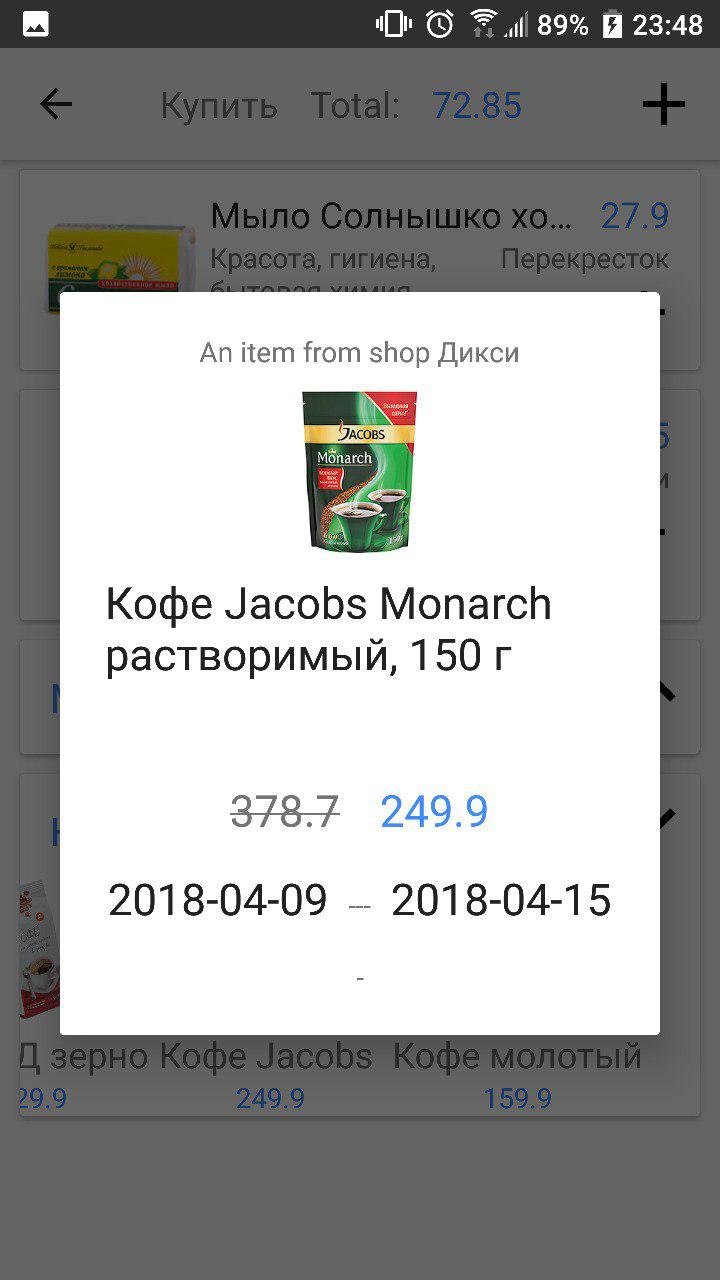
\includegraphics[height=0.38\textheight]{./screenshots/3/full_item_preview.jpg}
    \caption{\small{просмотр всей информации о товаре}}
    \endminipage{}
\end{figure}


Реализованa регистрация через мобильное приложение, реализован вход
в аккаунт через мобильное приложение, реализованa возможность смены аккаунта.

\begin{figure}[h!]
    \centering
    \minipage{0.45\textwidth}
    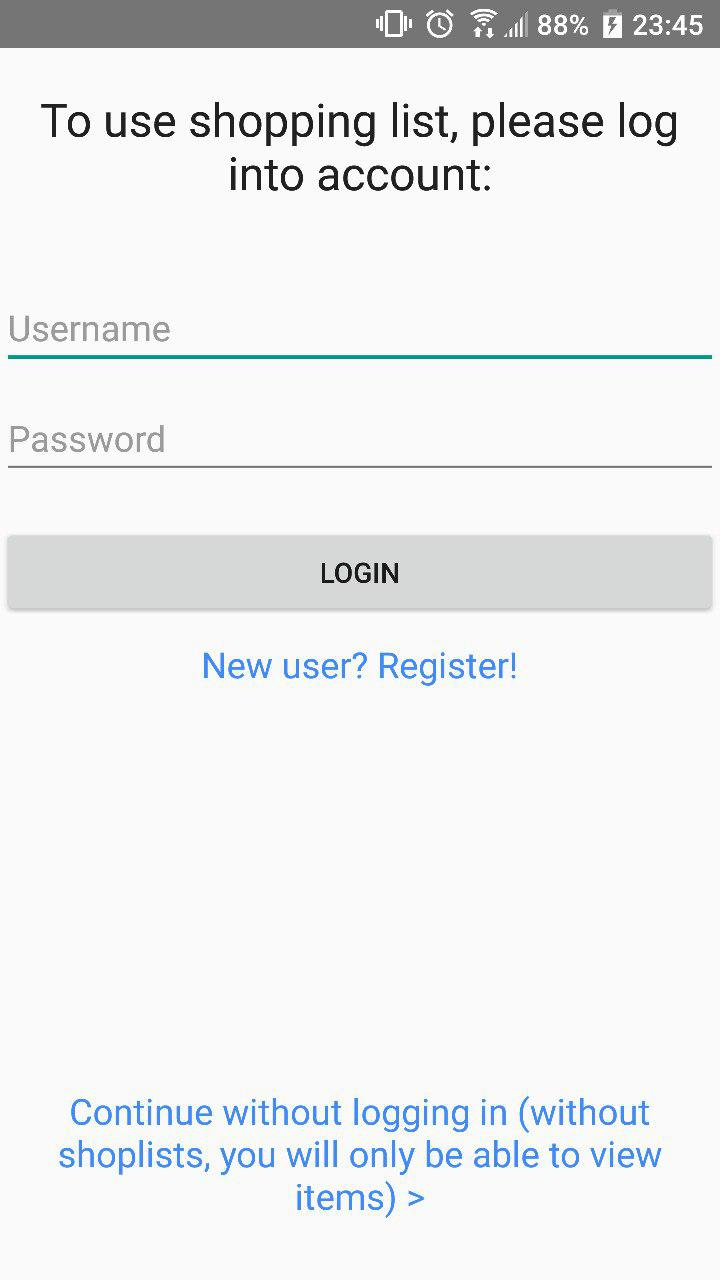
\includegraphics[height=0.42\textheight]{./screenshots/3/login.jpg}
    \caption{\small{вход в аккаунт}}
    \endminipage\hfill
    \minipage{0.45\textwidth}
    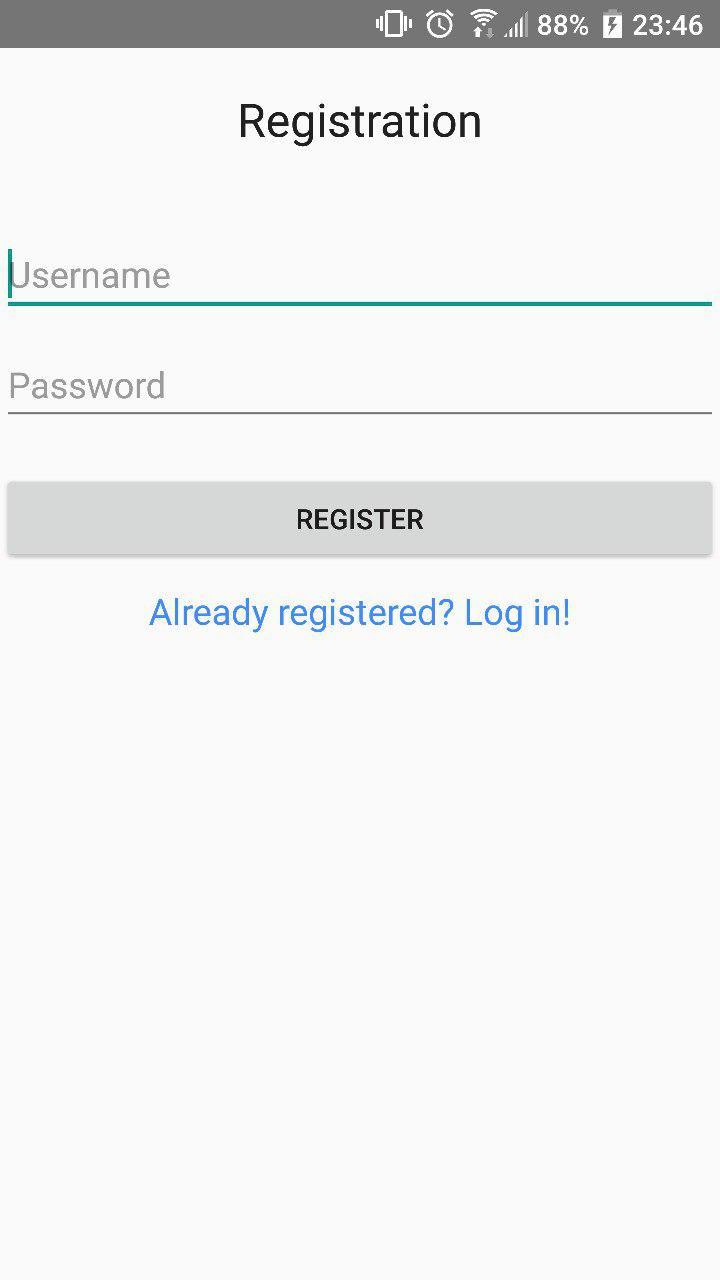
\includegraphics[height=0.42\textheight]{./screenshots/3/register.jpg}
    \caption{\small{регистрация аккаунта}}
    \endminipage{}
\end{figure}


Реализовано отображение всплывающих подсказок при долгом нажатии на элементы
управления button (кнопка), реализовано перенаправление в настройки сети для
последующего включения интернета при отсутствии интернет-соединения,
реализовано отображение индикатора процесса загрузки данных с сервера,
реализован обучающий фрагмент в разделе help, содержащий руководство
пользователя по управлению программой.

\begin{figure}[h!]
    \centering
    \minipage{0.3\textwidth}
    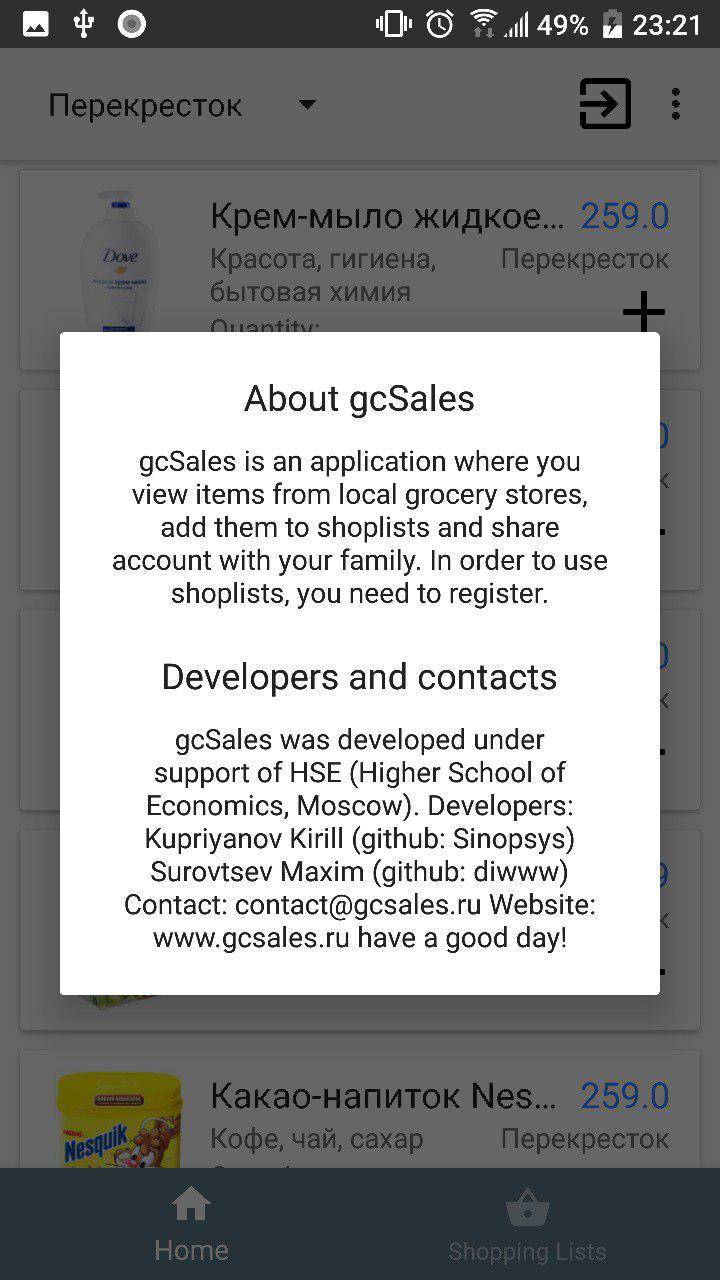
\includegraphics[height=0.38\textheight]{./screenshots/3/about.jpg}
    \caption{\small{просмотр раздела ``о приложении''}}
    \endminipage\hfill
    \minipage{0.3\textwidth}
    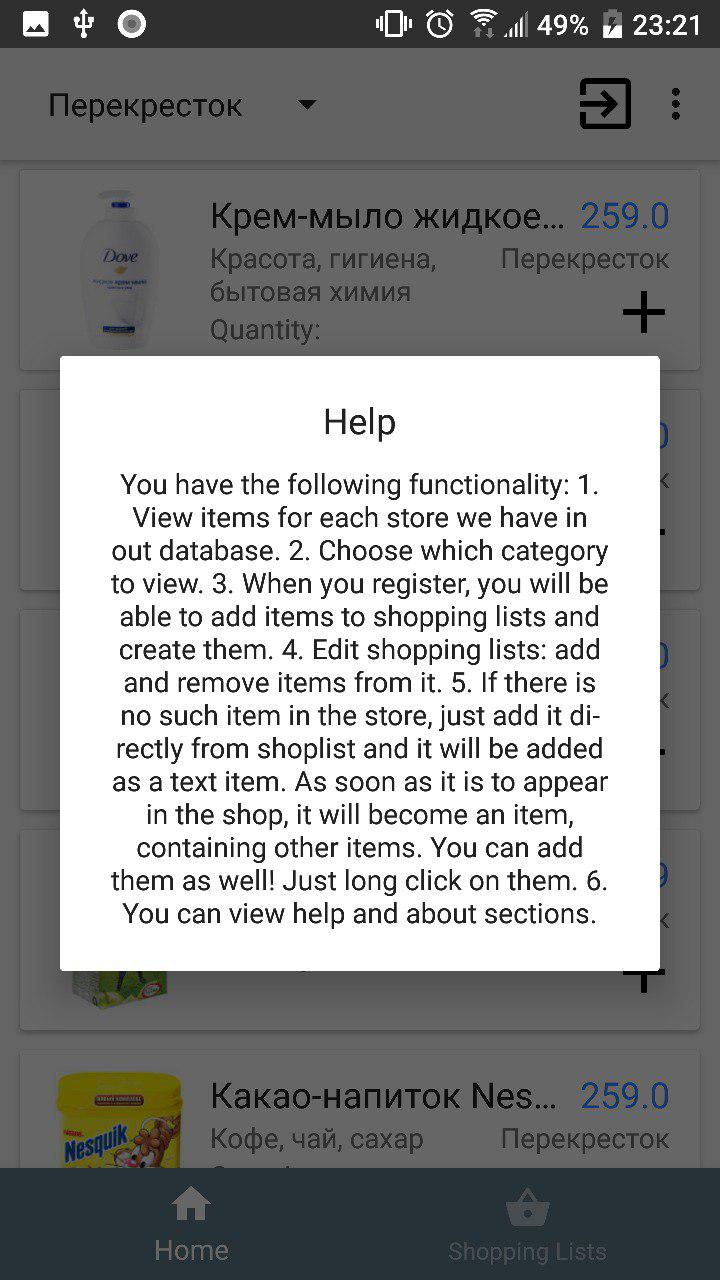
\includegraphics[height=0.38\textheight]{./screenshots/3/help.jpg}
    \caption{\small{просмотр подсказки пользования приложением}}
    \endminipage\hfill
    \minipage{0.3\textwidth}
    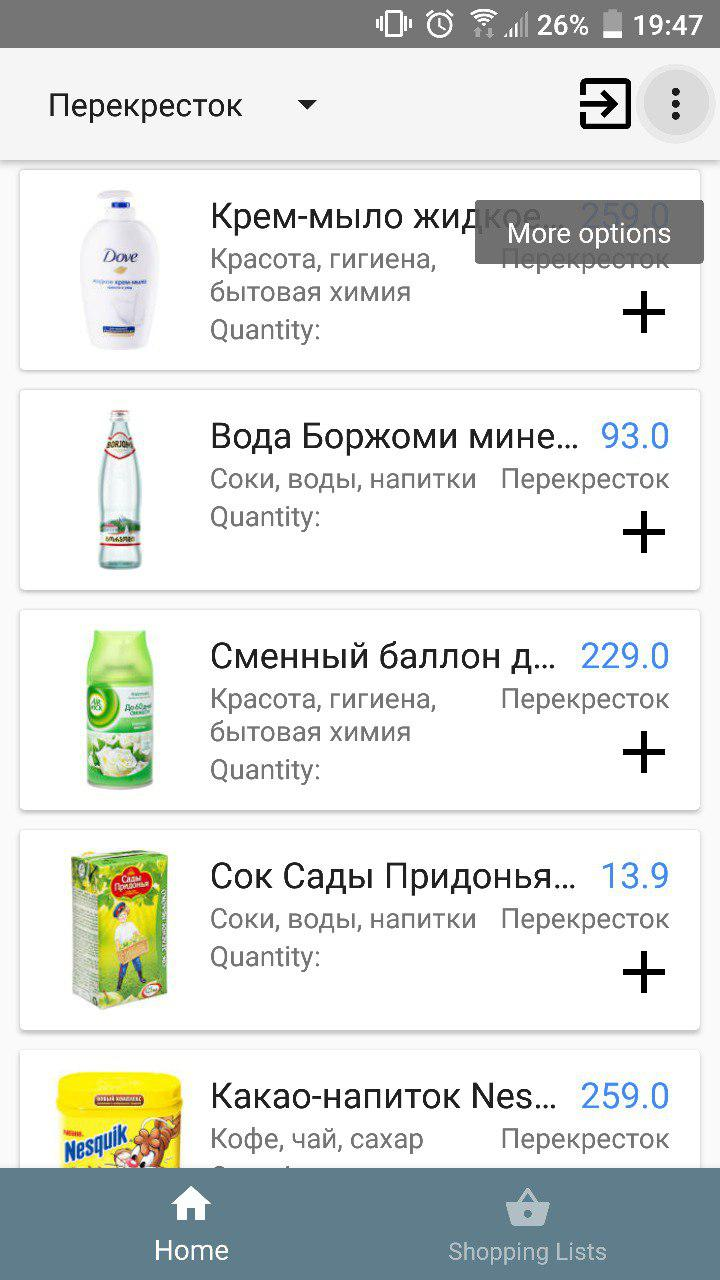
\includegraphics[height=0.38\textheight]{./screenshots/3/hint.jpg}
    \caption{\small{просмотр всплывающего описания элементов button (кнопок)}}
    \endminipage{}
\end{figure}

\subsubsection{Crawler}
Все необходимые для реализации программы модули реализованы (Рис.~\ref{tree})

\begin{figure}[h!]
    \centering
    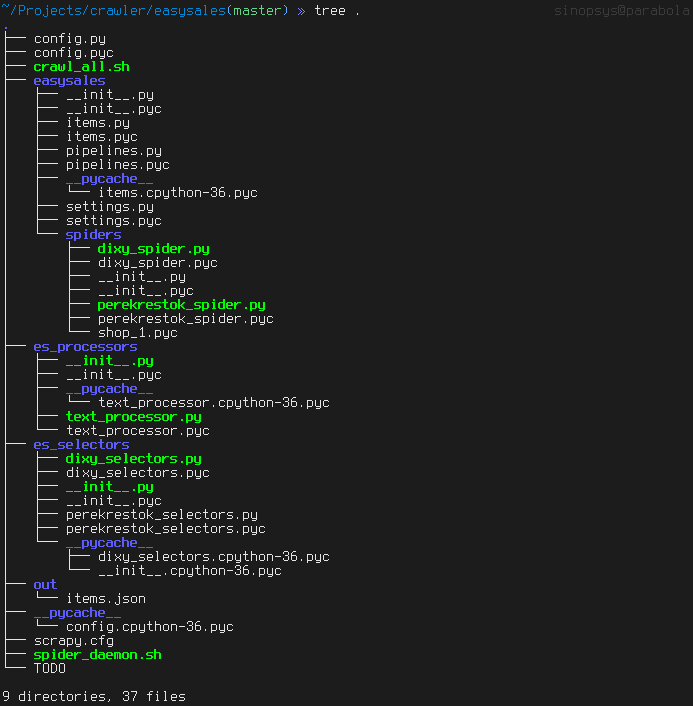
\includegraphics[width=0.9\textwidth]{./screenshots/3/tree.png}
    \caption{\small{структура проекта crawler'a}}
    \label{tree}
\end{figure}

Работа crawler'a на Рис.~\ref{crawl_dixy}. При запуске всё работает по описанному
в настоящей Пояснительной Записке алгоритму, отправляются запросы в базу
данных. Ошибок не наблюдается.

\begin{figure}[h!]
    \centering
    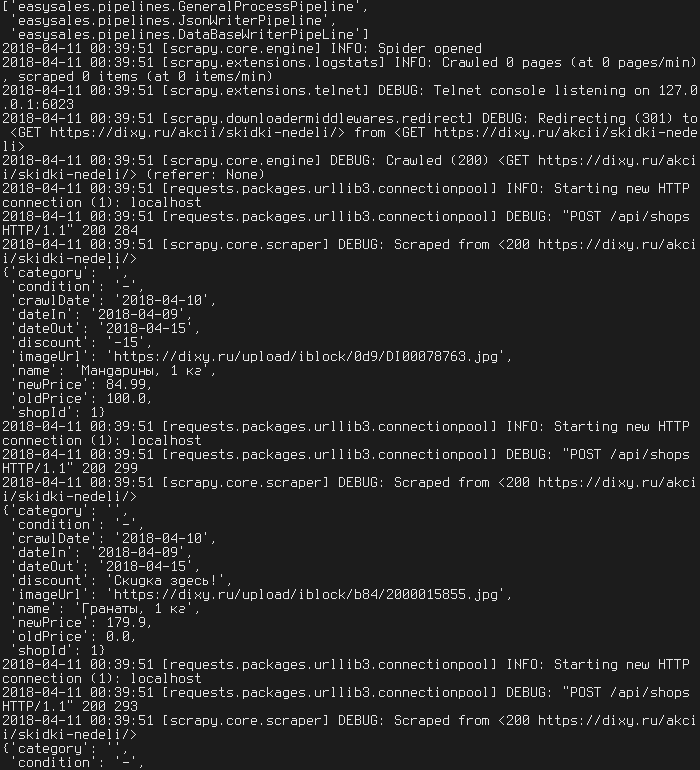
\includegraphics[width=0.9\textwidth]{./screenshots/3/crawl_dixy.png}
    \caption{\small{начало запуска crawler'a}}
    \label{crawl_dixy}
\end{figure}


\newpage
\subsection{Проверка требований к временным характеристикам}
\subsubsection{Андроид приложение}
Будут приводится log-сообщения (см. терминологию) из используемого средства разработки.

Время запуска приложения не превышает двух секунд:

\begin{figure}[h!]
    \centering
    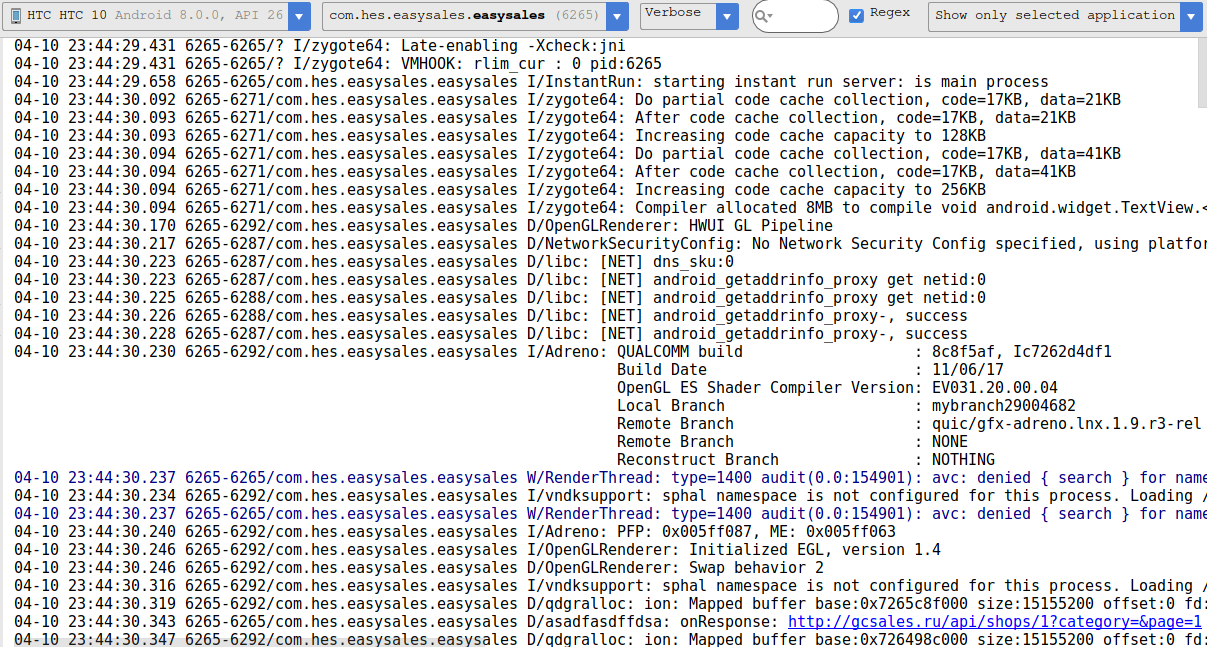
\includegraphics[width=0.9\textwidth]{./screenshots/3/lauch_log.png}
    \caption{\small{log. Запуск приложения}}
\end{figure}


Время загрузки одной страницы акций не превышает двух секунд:

\begin{figure}[h!]
    \centering
    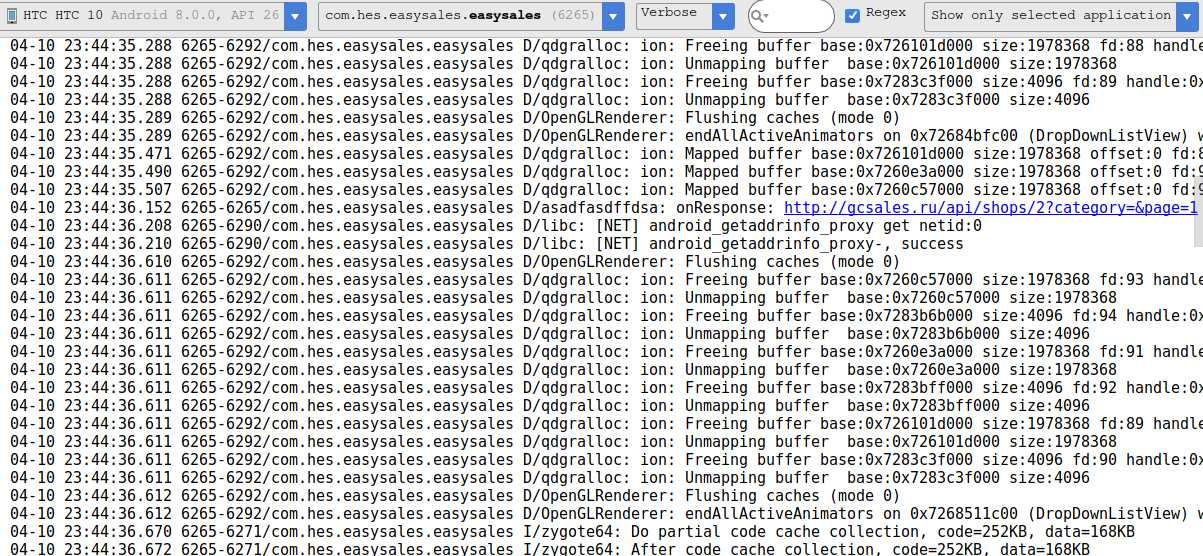
\includegraphics[width=0.9\textwidth]{./screenshots/3/load_log.png}
    \caption{\small{log. Загрузка акций}}
\end{figure}
Все временные требования соблюдены.
\subsubsection{Crawler}
Временные требования к работе crawler'a не предъявлялись.
